\section{Methodology: Decoupled Namespaces}
\label{sec:methodology-decoupled-namespaces}

\begin{figure}[tb]
\caption{Applications can decouple the namespace, write updates to a local
journal, and delay metadata updates.  Table~\ref{table:spectrum} shows how
these mechanisms (represented by the arrows) can be combined to provide weaker
consistency or durability semantics.  }\label{fig:decouple}
\centering
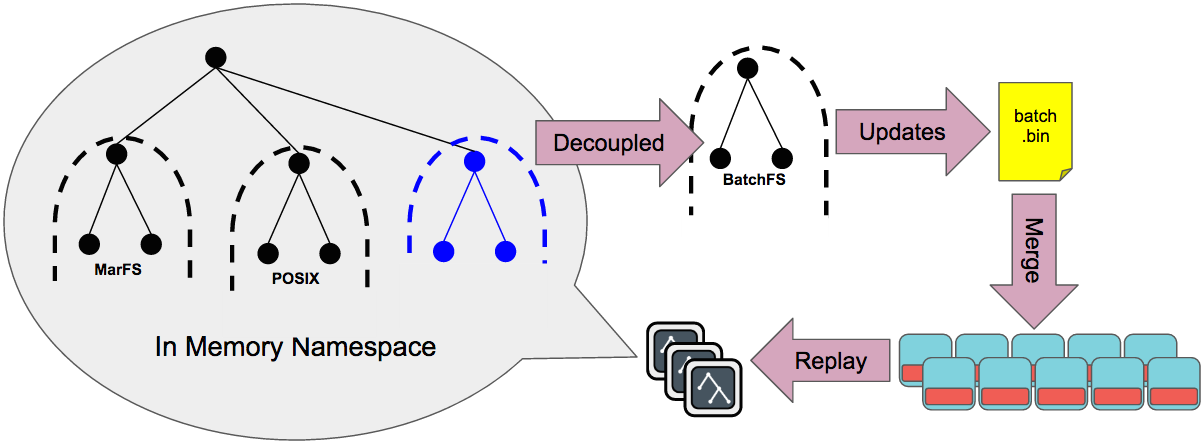
\includegraphics[width=90mm]{figures/fig-decouple.png}
\end{figure}

In this section we describe Cudele, our prototype system that lets future
programmers compose mechanisms (Section~\S\ref{sec:cudeles-mechanisms}) to
provide the necessary guarantees
(Section~\S\ref{sec:setting-policies-with-cudele}) for their application.

\subsection{Cudele's Mechanisms}
\label{sec:cudeles-mechanisms}

% describe the figure
Figure~\ref{fig:decouple} shows the mechanisms (labeled arrows) in Cudele and
which entity they are performed by (gray boxes). The metadata store and journal
are different ways of representing the namespace.  Cudele presents 6
mechanisms: RPCs, Stream, Create, Volatile Apply, Local Persist, and Global
Persist. ``RPCs" does round trip remote procedure calls to establish
consistency; it is the default implementation for complying with POSIX in
CephFS. ``Stream" has the metadata servers stream a journal of metadata updates
into the object store. ``Create" allows clients to append metadata events to an
in-memory journal. ``Volatile apply" takes the in-memory journal on the client
and applies it directly to the in-memory metadata store of the metadata server
cluster. ``Local Persist" takes the in-memory journal and writes it to the
client's disk. ``Global Persist" saves the journal as a an object in the object
store from the client.  Next, we discuss how these mechanisms can be composed
to get different consistency and durability semantics. 

%\begin{tabular}{ r | l }
%  \(\Rightarrow\)   & Description \\\hline
%  create            & events appended to in-memory journal \\
%  v\_apply           & journal volatily applied to in-memory metadata store \\
%  save              & journal saved to client's disk \\
%  persist           & journal saved in object store \\
%  replay            & metadata servers materialize namespace \\
%  RPCs              & round trip remote procedure calls \\
%  stream            & metadata server streams journal into RADOS \\
%\end{tabular}

\subsection{Setting Policies with Cudele}
\label{sec:setting-policies-with-cudele}

\begin{table}[t]
\begin{center}
\caption{Future programmers can explore the consistency (C) and
durability (D) spectrums by composing Cudele mechanisms. The consistency
and durability properties are not guaranteed until all mechanisms in the cell
are complete ({\it i.e.} the compositions should be considered atomic) and there are
no guarantees while tranisitioning between policies. \label{table:spectrum}}
\begin{tabular}{ l | l | l | l }
  C \(\rightarrow\) &&& \\  
  D \(\downarrow\)  	     & invisible         & weak        & strong  \\\hline
  none                       & create            & create          & RPCs    \\
                             &                   & +volatile apply &         \\\hdashline
  local                      & create            & create          & RPCs    \\
                             & +local persist    & +local persist  & +local  \\
                             &                   & +volatile apply &  persist\\\hdashline
  global                     & create            & create          & RPCs    \\
                             & +global persist   & +global persist & +stream \\
                             &                   & +volatile apply &         \\
\end{tabular}
\end{center}
\end{table}

% describe table
The spectrum of consistency and durability guarantees that adminstrators can
construct is shown in Table~\ref{table:spectrum}. The columns are the different
consistency semantics and the rows cover the spectrum of durability guarantees.
For consistency: ``invisible" means the system does not handle merging updates
into a global namespace and it is assumed that middleware or the application
manages consistency lazily; ``weak" merges updates at some time in the
future ({\it e.g.}, when the system has time, when number of updates reaches a
certain threshold, when the client is done writing, etc.); ; and updates in
``global" consistency are seen immediately by all clients. For durability,
``none" means that updates are volatile and will be lost on a failure. Stronger
guarantees are made with ``local", which means updates will be retained if the
client node recovers, and ``global", where all updates are always recoverable.

% which system they represent and which are impossible
Existing, state-of-the-art systems in HPC can be represented by the cells in
Table~\ref{table:spectrum}.  POSIX-compliant systems like CephFS and IndexFS
have global consistency and durability; DeltaFS uses ``invisible" consistency
and ``local" durability and BatchFS uses ``weak" consistency and ``local"
durability. These are just a few of the HPC examples.  

% how its done
To compose the mechanisms administrators inject which steps (described in
Section~\S\ref{sec:cudeles-mechanisms}) to run and which to use in parallel
using a domain specific language. For example, to get the semantics of BatchFS,
the administrator would inject the following pipeline:\\

\noindent \texttt{create+save+volatile apply}\\

% what is impossible
Although we can achieve all permutations of the different guarantees in
Table~\ref{table:spectrum}, not all of them make sense. For example, it
makes little sense to do \texttt{creates+RPCs} since both steps do the same
thing or \texttt{stream+save} since ``global" durability is stronger and has
more overhead than ``local" durability.  Formulaically, valid steps
include:\\

\noindent \texttt{<create|RPCs> [+v\_apply][+save][+persist][+stream]}

\subsection{Cudele Namespace API:\\Per-Subtree Policies}
\label{sec:cudele-namespace-api-per-subtree-policies}

% the interface
The interface for setting the subtree policies is with \{path,
\(<\)block\(|\)overwrite\(>\), pre-allocated inodes\} tuples. For example:

\texttt{(msevilla/mydir, policies.yml)}

would decouple the path \texttt{msevilla/mydir} and would apply the policies in
\texttt{policies.txt}. The policies file supports the following values:

\begin{itemize}

  \item \texttt{allocated\_inodes}: the number of inodes to allocate to the
  decoupled namespace (default 100)

  \item \texttt{interfere\_callback}: how to handle a request from another
  client targeted at the now decoupled subtree (default \texttt{block})

  \item \texttt{consistency\_callback}: which consistency model to use (default
  \texttt{RPCs})

  \item \texttt{durability\_callback}: which durability model to use (default
  \texttt{stream})

\end{itemize}

Given these default values decoupling the namespace with an empty policies file
would give the application 100 inodes but the subtree would behave like the
existing CephFS implementation. Table~\ref{table:spectrum} shows how one would use the Cudele
API to implement policies from related work. 


%

For \texttt{block}, any requests to this part of the namespace returns with
``Device is busy", which will spare the metadata server from wasting resources for updates
that may get overwritten. If the application does not mind losing updates, for
example it wants approximations for results that take too long to compute, it
can select \texttt{overwrite}. In this case, metadata will be written and the
computation from the decoupled namespace will take priority at merge time because the results
are more accurate.

\begin{listing}
\begin{minted}[frame=single,
               framesep=3mm,
               xleftmargin=21pt,
               tabsize=4]{js}
{     
    "allocated_inodes": "100000"
    "interfere_policy": "block"
    "consistency": "create"
    "durability": "local_persist"
}
\end{minted}
\caption{Implementing DeltaFS with Cudele.}
\label{src:deltafs}
\end{listing}

\begin{listing}
\begin{minted}[frame=single,
               framesep=3mm,
               xleftmargin=21pt,
               tabsize=4]{js}
{     
    "allocated_inodes": "100000"
    "interfere_policy": "block"
    "consistency": "create+volatile_apply"
    "durability": "local_persist"
}
\end{minted}
\caption{Implementing BatchFS with Cudele.}
\label{src:batchfs}
\end{listing}

\begin{listing}
\begin{minted}[frame=single,
               framesep=3mm,
               xleftmargin=21pt,
               tabsize=4]{js}
{     
    "allocated_inodes": "-"
    "interfere_policy": "-"
    "consistency": "RPCs"
    "durability": "stream"
}
\end{minted}
\caption{Existing CephFS on Cudele.}
\label{src:batchfs}
\end{listing}

\subsection{Programmability Approach}

% what is programmability
A programmable storage system exposes internal subsystem as building blocks for
higher level services. This `dirty-slate' approach limits redundant code and
leverages the robustness of the underlying storage system. Cudele uses this
approach and re-uses some of the building blocks from the Malacology
programmable storage system~\cite{sevilla:eurosys17} to great success and
requires only:

\begin{itemize}

  \item 354 lines of library code

  \item 219 lines of non-destructive metadata server code, which is not used
  unless it is turned on

  \item 4 lines of destructive client/server code to check whether a namespace
  is decoupled

\end{itemize}

% how it works in CephFS, how I used it
\subsubsection{Metadata Store}
\label{sec:metadata-store}

% how it works in CephFS
In CephFS, the metadata store is a data structure that represents the file
system namespace. This data structure is stored in two places: in memory ({\it
i.e.} in the collective memory of the metadata server cluster) and as objects
in the object store. In the object store, directories and their inodes are
stored together in objects to improve the performance of scans.  The metadata
store data structure is structured as a tree of directory fragments making it
easier to read and traverse.\\

% how i used it
\noindent\textbf{Cudele}: uses the metadata store format to write objects
formatted like the journal into the object store. By writing with the same
format, the metadata servers can read and use the recovery code to materialize
the updates from a client's decoupled namespace ({\it i.e.} merge).

\subsubsection{Journal}
\label{sec:journal}

The journal is the second way that CephFS represents the file system namespace;
it is a log of metadata updates that can materialize the namespace when the
updates are replayed onto the metadata store. The journal is a ``pile system";
writes are fast but reads are slow because state must be reconstructed.
Specifically, reads are slow because there is more state to read, it is
unorganized, and many of the updates may be redundant.\\

\noindent\textbf{Cudele}: uses the journal subsystems within the metadata
server to replay updates onto the in-memory metadata store.  When the clients
are ready to merge their updates back into the global namespace, they pass a
binary file of  metadata updates to the metadata server. The metadata server
uses its recovery code to ``replay" the updates. 

\subsubsection{Journal Tool}
\label{sec:journal-tool}

The journal tool is used for disaster recovery and lets administrators view and
modify the journal. It can read the journal, export the journal as a file,
erase events, and apply updates to the metadata store.  To apply journal
updates to the metadata store, the journal tool reads the journal from object
store objects and replays the updates on the metadata store in the object
store.\\

\noindent\textbf{Cudele}: using the journal tool, clients can materialize the
journal in memory and append events to their own copy. When they are done they
export their journal to a binary file. Clients also use the journal tool to
save their updates to disk or to the object store.


% Journal import
%The journal tool imports journals from binary files stored on disk.  First the
%header of the dump is sanity checked and written into RADOS to the ``header"
%object.  The ``header" object has metadata about the journal as well as the
%locations of all the journal pointers (e.g., where the tail of the journal is,
%where we are currently trimming, etc.).  Then the journal events are cleaned
%(erasing trailing events that are not part of the header) and written as
%objects into RADOS.  Note that while the journal is in RADOS, the metadata
%servers do do not have the namespace reconstructed in memory so the metadata
%cluster will not service requests relating to the journal of imported events.
%To construct the namespace in the collective memory of the metadata servers we
%need to first construct the namespace in RADOS. The journal tool can explicitly
%do this by  applying the journal to the metadata store in RAODS. This will pull
%the objects containing journal segments and replay them on the metadata store.
%Finally, we delete the journal in RADOS and restart the metadata servers so
%they rebuild their caches.

% Journal export
%First the
%journal is scanned for the header and then journal is recovered. To recover the
%journal the ``header" object is read off disk and then objects are probed in
%order and starting from the write position saved in the header. Probing will
%update the write position if it finds objects with data in them. 

% Journal export
%When exporting a journal of events, the journal tool first scans the journal to
%check for corruption. Then it recovers the journal by reading the ``header"
%object out of RADOS.  After reading the header, the journal tool can pull
%journal segments from RADOS because it knows how many objects to pull and how
%far to seek within those objects.

%% The data structures
%The metadata that the event touches, including inodes, paths, and timestamps,
%are stored as metablobs. Each piece of metadata inside a metablob is called a
%dirlump. A dump has a section for lumps (dirfrag, dirlump), roots (dentries),
%table client transactions (tid, version), renamed directory fragments (maps,
%versions, alloc/preallocated inodes), inodes starting a truncate, inodes
%finishing a truncate, destroyed inodes, and client requests. Unfortunately for
%me (and you since you are reading this paper), this does not make any sense.
%
%Each directory fragment has an associated directory lump, which is just a bunch
%of metadata. The most interesting part of the dirlump is the fullbits array,
%which has a dentry OR inode. To walk the tree, iterate over all the dirlumps
%and then all the full bits, saving off the children and inode locations. The
%children tell us which dentry names an inode has and the inode locations map
%the parent inode to its child inode and dentry.  

\subsubsection{Inode Cache}
\label{sec:inode-cache}

In CephFS, the inode cache reduces the number of RPCs between clients and
metadata servers. Without contention clients can resolve metadata reads locally
thus reducing operations like \texttt{lookup()}.  For example, if a client or
metadata server is not caching the directory inode, all creates within that
directory will result in a lookup and a create request. If the directory inode
is cached then only the create needs to be sent.  The size of the inode cache
is configurable so as not to saturate the memory on the metadata server --
inodes in CephFS are about 1400
bytes\footnote{http://docs.ceph.com/docs/jewel/dev/mds\_internals/data-structures/}.
The inode cache has code for manipulating inode numbers, such as pre-allocating
inodes to clients.\\

\noindent\textbf{Cudele}: uses the internal inode cache code to allocate inodes
to clients that decouple parts of the namespace and to skip inodes used by the
client at merge time.

\subsubsection{Large Inodes}
\label{sec:large-inodes}

In CephFS, inodes store policies for policies, like how the file is striped
across the object store or for managing subtrees for load balancing. These
policies adhere to logical partitionings of metadata or data, like Ceph pools and file
system namespace subtrees. To implement this, the namespace data structure has
the ability to recursively apply policies to subtrees and to isolate subtrees
from each other.  \\

\noindent\textbf{Cudele}: uses the large inodes to store consistency and
durability policies in the directory inode. This approach uses the File Type
interface from the Malacology programmable store
system~\cite{sevilla:eurosys17} and it tells clients how to access the
underlying metadata. The underlying implementation stores executable code in
the inode that calls the different Cudele mechanisms. Of course, there are many
security and access control aspects of this approach but that is beyond the
scope of this paper.

% lead into implementation


% // limit consistency
% if metadata write (create) -- try to reduce error bars for many creates and runtime of one touch)
%   if !RPCs
%     if overwrite
%       do nothing and let the RPC go
%     else
%       return -EBUSY
%
% // limit durability
% if !stream
%   return immediately on mdlog


